\documentclass{article}
\usepackage[utf8]{inputenc}
\usepackage{setspace}
\usepackage{tikz}
\usetikzlibrary{positioning}
\usepackage{amsfonts}
\usepackage{amssymb}
\usepackage{amsmath}
\usepackage{amsthm}
\usepackage{systeme}
\usepackage{mathtools}
\usepackage{hyperref}
\usepackage{venndiagram}
\usepackage{pgfplots}
\usetikzlibrary{pgfplots.statistics}
\pgfplotsset{compat=newest}



\begin{document}
\section*{Question 1}

~

\subsection*{a}

~

\begin{align*}
    &\#\mathrm{bin}\approx \sqrt{129}\approx 12\\
    \Rightarrow&\#\mathrm{bin}=12\\
    &\mathrm{bin\_width}=\frac{\max-\min}{\#\mathrm{bin}}=\frac{18.9-2.2}{12}\approx1.4\\
    &\mathrm{bin}_1=\{a,a\in[2.2,3.6)\}\\
    &V_{\mathrm{bin}_1}=7\\
    &f_{\mathrm{bin}_1}=7\div1.4=5\\ 
    &\mathrm{bin}_2=\{a,a\in[3.6,5.0)\}\\
    &V_{\mathrm{bin}_2}=13\\
    &f_{\mathrm{bin}_2}=13\div1.4\approx9.29\\ 
    &\mathrm{bin}_3=\{a,a\in[5.0,6.4)\}\\
    &V_{\mathrm{bin}_3}=28\\
    &f_{\mathrm{bin}_3}=28\div1.4=20\\ 
    &\mathrm{bin}_4=\{a,a\in[6.4,7.8)\}\\
    &V_{\mathrm{bin}_4}=30\\
    &f_{\mathrm{bin}_4}=30\div1.4\approx21.43\\ 
    &\mathrm{bin}_5=\{a,a\in[7.8,9.2)\}\\
    &V_{\mathrm{bin}_5}=11\\
    &f_{\mathrm{bin}_5}=11\div1.4\approx7.86\\ 
    &\mathrm{bin}_6=\{a,a\in[9.2,10.6)\}\\
    &V_{\mathrm{bin}_6}=20\\
    &f_{\mathrm{bin}_6}=20\div1.4\approx14.29\\
    &\mathrm{bin}_7=\{a,a\in[10.6,12.0)\}\\
    &V_{\mathrm{bin}_7}=10\\
    &f_{\mathrm{bin}_7}=10\div1.4\approx7.14\\ 
    &\mathrm{bin}_8=\{a,a\in[12.0,13.4)\}\\
    &V_{\mathrm{bin}_8}=2\\
    &f_{\mathrm{bin}_8}=2\div1.4=\approx1.43\\ 
    &\mathrm{bin}_9=\{a,a\in[13.4,14.8)\}\\
    &V_{\mathrm{bin}_9}=3\\
    &f_{\mathrm{bin}_9}=3\div1.4\approx2.14\\ 
\end{align*}

\begin{align*}
    &\mathrm{bin}_{10}=\{a,a\in[14.8,16.2)\}\\
    &V_{\mathrm{bin}_{10}}=4\\
    &f_{\mathrm{bin}_{10}}=4\div1.4\approx2.86\\ 
    &\mathrm{bin}_{11}=\{a,a\in[16.2,17.6)\}\\
    &V_{\mathrm{bin}_{11}}=0\\
    &f_{\mathrm{bin}_{11}}=0\div1.4=0\\ 
    &\mathrm{bin}_{12}=\{a,a\in[17.6,19.0)\}\\
    &V_{\mathrm{bin}_{12}}=1\\
    &f_{\mathrm{bin}_{12}}=1\div1.4\approx0.71\\ 
\end{align*}

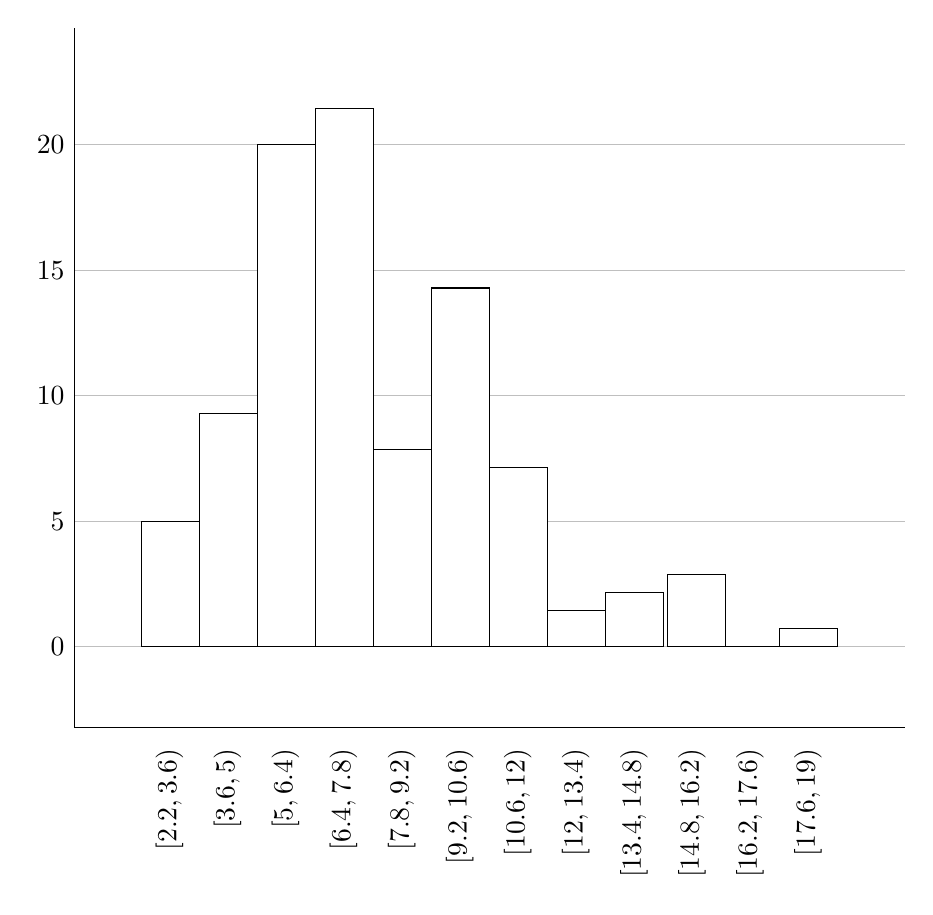
\begin{tikzpicture}
    \begin{axis}[
        ybar, bar width=1.4,
        ymajorgrids,
        axis lines*= left,
        width=\linewidth,
        xtick style= {draw=none}, ytick style= {draw=none},
        enlargelimits=0.15,
        xtick={2.2, 3.6, 5.0, 6.4, 7.8, 9.2, 10.6, 12.0, 13.4, 14.8, 16.2, 17.6, 19.0},
        x tick label style = {rotate=90, yshift=2.5ex},
        x tick label as interval=true,
        xticklabel={$[\pgfmathprintnumber{\tick}, \pgfmathprintnumber{\nexttick})$},
        x tick label style = {/pgf/number format/set thousands separator={.}},
        y tick label style = {/pgf/number format/set thousands separator={\,}},
                 ]  
        \addplot[ybar, fill=white] coordinates {(2.2,5) (3.6,9.29) (5.0,20) (6.4,21.43) (7.8,7.86) (9.2,14.29) (10.6,7.14) (12.0,1.43) (13.4,2.14) (14.9,2.86) (16.2,0) (17.6,0.71)};   
    \end{axis}
\end{tikzpicture}

\subsection*{b}

~

The typical value should be median since the date values are not symmetrical and have outliers.$\mathrm{Med
}=7$. So the typical value is 7.

~

\subsection*{c}

~

The display is spread out because there is a wide range of values and there are data points.

~

\subsection*{d}

~

\begin{align*}
    &\mathrm{Med }=7\\
    &\mathrm{Mean }=\frac{\sum(x_i)}{129}\approx7.7\\
    \Rightarrow&\mathrm{Med}<\mathrm{Mean}\\
    \Rightarrow&\text{Right-skewed}\\
\end{align*}

~

\subsection*{e}

~

\begin{align*}
    &Q_1=(5.6+5.6)\div2=5.6\\
    &Q_3=(8.8+9.0)\div2=8.9\\
    &\mathrm{IQR}=Q_3-Q_1=3.3\\
    &Q_1-1.5\mathrm{IQR}=5.6-4.95=0.65\\
    &Q_3+1.5\mathrm{IQR}=8.9+4.95=13.85\\
    &\mathrm{Outliers}=\{x,x\in(-\infty,0.65)\cup(13.85,\infty)\}\\
    \Rightarrow&\mathrm{Outliers}=\{14.3,14.6,15,15,15.3,15.5,18.9\}\\
    &\text{There is no outliers smaller than the median, but are outliers larger than the median}\\
\end{align*}

\newpage

\section*{Question 2}

~

There exists negative value for the x-axis, meaning that there are people speeding up during 35km-40km.The time differences range from -50 to 750 sec. The most frequent classes are 50 to 150,meaning that most runners are 50 to 150 seconds slower. The diagram is skew to the right, so the mean is greater than the median.

\newpage

\section*{Question 3}

~

\subsection*{a}

~

\begin{align*}
    &\overline{x}=\frac{\sum x_i}{n}=\frac{116.4+115.9+114.6+115.2+115.8}{5}=115.58\\
    &x_1-\overline{x}=116.4-115.58=0.82\\
    &x_2-\overline{x}=115.9-115.58=0.32\\
    &x_3-\overline{x}=114.6-115.58=-0.98\\
    &x_4-\overline{x}=115.2-115.58=-0.38\\
    &x_5-\overline{x}=115.8-115.58=0.22\\
\end{align*}

~

\subsection*{b}

~

\begin{align*}
    &s^2\frac{0.82^2+0.32^2+0.98^2+0.38^2+0.22^2}{4}=0.482\\
    &s=\sqrt{s^2}\approx0.694\\
\end{align*}

~

\subsection*{c}

~

\begin{align*}
    &S_{xx}=\sum{x_i}^2-\frac{(\sum x_i)^2}{n}\\
    &=66795.61-\frac{577.9^2}{5}\\
    &=1.928\\
    &s^2=\frac{S_{xx}}{4}=0.482\\
\end{align*}

~

\subsection*{d}

~

\begin{align*}
    &{x_1}'=116.4-100=16.4\\
    &{x_2}'=115.9-100=15.9\\
    &{x_3}'=114.6-100=14.6\\
    &{x_4}'=115.2-100=15.2\\
    &{x_5}'=115.8-100=15.8\\
    &\overline{x'}=15.58\\
    &{x_1}'-\overline{x'}=16.4-15.58=0.82\\
    &{x_2}'-\overline{x'}=15.9-15.58=0.32\\
    &{x_3}'-\overline{x'}=14.6-15.58=-0.98\\
    &{x_4}'-\overline{x'}=15.2-15.58=-0.38\\
    &{x_5}-\overline{x'}=15.8-15.58=0.22\\
    &{s'}^2=\frac{0.82^2+0.32^2+0.98^2+0.38^2+0.22^2}{4}=0.482\\
    \Rightarrow&\text{Variance stays the same when the whole data set is added or subtracted a certain value}\\
\end{align*}

\newpage

\section*{Question 4}

~

The two sets of data have similar medians. Machine 2 has a wider range and a larger IQR than machine 1. Machine 2 ranges from 85 to 115 roughly,with IQR about 20, but machine 1 has much smaller range and IQR. There is an outlier in machine 1 but no outlier in machine 2. Also, it is easy to see that the data of machine 1 is closer to the 

In conclusion, I think machine 1 has a stabler performance than machine 2.

\newpage

\section*{Question 5}

~

\begin{align*}
    &\min=55.3\\
    &\max=83\\
    &\text{Median }=64.7\\
    &\text{Mean }=64.89\\
    &Q_1=57.8\\
    &Q_3=70.4\\
    &IQR=Q_3-Q_1=12.6\\
    &\text{Range }=\max-\min=27.7\\
    &\text{Median }+1.5IQR=83.6>\max\\
    &\text{Median }-1.5IQR=45.8<\min\\
\end{align*}

According to the date, mean is greater than median, which means that the histogram should be right-skewed. The maximum is smaller than Median+1.5 IQR, and the minimum is bigger than Median-1.5 IQR, this means that there is no outlier in this set of data.

\newpage

~

\subsection*{a}

~

\begin{align*}
    &\min=15\\
    &\max=829\\
    &\text{Median }=\frac{195+196}{2}=195.5\\
    &\text{Mean }=\frac{\sum x_i}{n}=\frac{22198}{100}=221.98\\
    &Q_1=\frac{124+131}{2}=127.5\\
    &Q_3=\frac{282+284}{2}=283\\
    &\text{Range }=829-15=814\\
    &IQR=Q_3-Q_1=283-127.5=155.5\\
\end{align*}

~

\subsection*{b}

~

\begin{align*}
    &s^2=\frac{\sum(x-\overline{x})^2}{n-1}=\frac{2070524}{99}\approx 20914.384\\
    &s=\sqrt{s^2}\approx144.618\\
\end{align*}

~

\subsection*{c}

~

\begin{align*}
    &Q_1-1.5IQR=127.5-1.5\times 155.5=-105.75\\
    &Q_3+1.5IQR=283+1.5\times 155.5=516.25\\
    \Rightarrow&x\text{ is an outlier }\Leftrightarrow x\in(-\infty,-105.75)\cup(516.25,\infty)\\
\end{align*}

~

\subsection*{d}

~

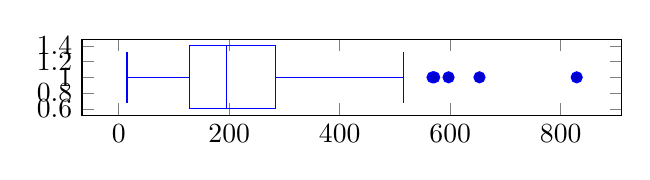
\begin{tikzpicture}
    \begin{axis}[y=1cm]
        \addplot+[
            boxplot prepared={
                lower whisker=15,
                lower quartile=127.5,
                median=195.5,
                upper quartile=283,
                upper whisker=516.25,   
            },
        ]
        table [row sep =\\,y index =0]{
            data \\568\\571\\597\\653\\829\\
        };
    \end{axis}
\end{tikzpicture}

~

\subsection*{e}

~

The distribution is right skewed, can be seen from the fact that the mean is bigger than the median. There are five outliers in this set of data. Those big numbers are the cause of the right-shift of the mean. And because of those outliers, median is the better way of representing the center instead of mean. So the data ranges at [15,497] and center at 195.5, excluding the outliers. It's IQR is 155.5, and its standard deviation is 144.618.
\end{document}